\documentclass[tikz,border=3mm]{standalone}
% based on an answer by user http://tex.stackexchange.com/users/1952/ignasi
% on http://tex.stackexchange.com/questions/174317/creating-a-labeled-tetrahedron-with-tikzpicture
\begin{document}
\tikzset{>=latex}
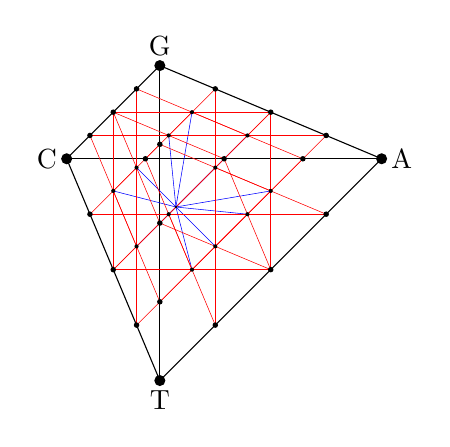
\begin{tikzpicture}[line join = round, line cap = round]
\pgfmathsetmacro{\xfactor}{1};
\pgfmathsetmacro{\yfactor}{1};
\pgfmathsetmacro{\zfactor}{.75/sqrt(2)};
\coordinate [label=right:A] (A) at ( 2*\xfactor,  0*\yfactor, -2*\zfactor);
\coordinate [label=left:C]  (C) at (-2*\xfactor,  0*\yfactor, -2*\zfactor);
\coordinate [label=above:G] (G) at ( 0*\xfactor,  2*\yfactor,  2*\zfactor);
\coordinate [label=below:T] (T) at ( 0*\xfactor, -2*\yfactor,  2*\zfactor);

\coordinate [] (AACC) at  ( 0*\xfactor,  0*\yfactor, -2*\zfactor);
\coordinate [] (AAGG) at  ( 1*\xfactor,  1*\yfactor,  0*\zfactor);
\coordinate [] (AATT) at  ( 1*\xfactor, -1*\yfactor,  0*\zfactor);
\coordinate [] (CCGG) at  (-1*\xfactor,  1*\yfactor,  0*\zfactor);
\coordinate [] (CCTT) at  (-1*\xfactor, -1*\yfactor,  0*\zfactor);
\coordinate [] (GGTT) at  ( 0*\xfactor,  0*\yfactor, 2*\zfactor);

\coordinate [] (AAAC) at  ( 1*\xfactor,  0*\yfactor, -2*\zfactor);
\coordinate [] (ACCC) at  ( -1*\xfactor,  0*\yfactor, -2*\zfactor);
\coordinate [] (AAAG) at  ( 1.5*\xfactor,  0.5*\yfactor, -1*\zfactor);
\coordinate [] (AGGG) at  ( 0.5*\xfactor,  1.5*\yfactor, 1*\zfactor);
\coordinate [] (AAAT) at  ( 1.5*\xfactor, -0.5*\yfactor, -1*\zfactor);
\coordinate [] (ATTT) at  ( 0.5*\xfactor,  -1.5*\yfactor,  1*\zfactor);
\coordinate [] (CCCG) at  ( -1.5*\xfactor,  .5*\yfactor, -1*\zfactor);
\coordinate [] (CGGG) at  ( -0.5*\xfactor,  1.5*\yfactor, 1*\zfactor);
\coordinate [] (CCCT) at  ( -1.5*\xfactor,  -0.5*\yfactor, -1*\zfactor);
\coordinate [] (CTTT) at  ( -0.5*\xfactor,  -1.5*\yfactor, 1*\zfactor);
\coordinate [] (GGGT) at  ( 0*\xfactor, 1*\yfactor, 2*\zfactor);
\coordinate [] (GTTT) at  ( 0*\xfactor,  -1*\yfactor,  2*\zfactor);


\coordinate [] (AACG) at (0.5*\xfactor, 0.5*\yfactor, -1.0*\zfactor);
\coordinate [] (ACCG) at (-0.5*\xfactor, 0.5*\yfactor, -1.0*\zfactor);
\coordinate [] (ACGG) at (0.0*\xfactor, 1.0*\yfactor, 0.0*\zfactor);
\coordinate [] (AACT) at (0.5*\xfactor, -0.5*\yfactor, -1.0*\zfactor);
\coordinate [] (ACCT) at (-0.5*\xfactor, -0.5*\yfactor, -1.0*\zfactor);
\coordinate [] (ACTT) at (0.0*\xfactor, -1.0*\yfactor, 0.0*\zfactor);
\coordinate [] (AAGT) at (1.0*\xfactor, 0.0*\yfactor, 0.0*\zfactor);
\coordinate [] (AGGT) at (0.5*\xfactor, 0.5*\yfactor, 1.0*\zfactor);
\coordinate [] (AGTT) at (0.5*\xfactor, -0.5*\yfactor, 1.0*\zfactor);
\coordinate [] (CCGT) at (-1.0*\xfactor, 0.0*\yfactor, 0.0*\zfactor);
\coordinate [] (CGGT) at (-0.5*\xfactor, 0.5*\yfactor, 1.0*\zfactor);
\coordinate [] (CGTT) at (-0.5*\xfactor, -0.5*\yfactor, 1.0*\zfactor);

\coordinate [] (ACGT) at (0*\xfactor, -0*\yfactor, 1*\zfactor);

\draw[opacity=1] (A) -- (AAAC);
\draw[opacity=1] (AAAC) -- (AACC);
\draw[opacity=1] (AACC) -- (ACCC);
\draw[opacity=1] (ACCC) -- (C);
\draw[opacity=1] (A) -- (AAAG);
\draw[opacity=1] (AAAG) -- (AAGG);
\draw[opacity=1] (AAGG) -- (AGGG);
\draw[opacity=1] (AGGG) -- (G);
\draw[opacity=1] (A) -- (AAAT);
\draw[opacity=1] (AAAT) -- (AATT);
\draw[opacity=1] (AATT) -- (ATTT);
\draw[opacity=1] (ATTT) -- (T);
\draw[opacity=1] (C) -- (CCCG);
\draw[opacity=1] (CCCG) -- (CCGG);
\draw[opacity=1] (CCGG) -- (CGGG);
\draw[opacity=1] (CGGG) -- (G);
\draw[opacity=1] (C) -- (CCCT);
\draw[opacity=1] (CCCT) -- (CCTT);
\draw[opacity=1] (CCTT) -- (CTTT);
\draw[opacity=1] (CTTT) -- (T);
\draw[opacity=1] (G) -- (GGGT);
\draw[opacity=1] (GGGT) -- (GGTT);
\draw[opacity=1] (GGTT) -- (GTTT);
\draw[opacity=1] (GTTT) -- (T);

\draw[blue, opacity=1, very thin] (AACG) -- (ACGT);
\draw[blue, opacity=1, very thin] (ACCG) -- (ACGT);
\draw[blue, opacity=1, very thin] (ACGG) -- (ACGT);
\draw[blue, opacity=1, very thin] (AACT) -- (ACGT);
\draw[blue, opacity=1, very thin] (ACCT) -- (ACGT);
\draw[blue, opacity=1, very thin] (ACTT) -- (ACGT);
\draw[blue, opacity=1, very thin] (AAGT) -- (ACGT);
\draw[blue, opacity=1, very thin] (AGGT) -- (ACGT);
\draw[blue, opacity=1, very thin] (AGTT) -- (ACGT);
\draw[blue, opacity=1, very thin] (CCGT) -- (ACGT);
\draw[blue, opacity=1, very thin] (CGGT) -- (ACGT);
\draw[blue, opacity=1, very thin] (CGTT) -- (ACGT);

\draw[red, opacity=1, very thin] (AACG) -- (AAAC);
\draw[red, opacity=1, very thin] (AACG) -- (AAAG);
\draw[red, opacity=1, very thin] (AACG) -- (AACC);
\draw[red, opacity=1, very thin] (AACG) -- (AAGG);
\draw[red, opacity=1, very thin] (AACG) -- (ACCG);
\draw[red, opacity=1, very thin] (AACG) -- (ACGG);
\draw[red, opacity=1, very thin] (ACCG) -- (AACC);
\draw[red, opacity=1, very thin] (ACCG) -- (AACG);
\draw[red, opacity=1, very thin] (ACCG) -- (ACCC);
\draw[red, opacity=1, very thin] (ACCG) -- (ACGG);
\draw[red, opacity=1, very thin] (ACCG) -- (CCCG);
\draw[red, opacity=1, very thin] (ACCG) -- (CCGG);
\draw[red, opacity=1, very thin] (ACGG) -- (AACG);
\draw[red, opacity=1, very thin] (ACGG) -- (AAGG);
\draw[red, opacity=1, very thin] (ACGG) -- (ACCG);
\draw[red, opacity=1, very thin] (ACGG) -- (AGGG);
\draw[red, opacity=1, very thin] (ACGG) -- (CCGG);
\draw[red, opacity=1, very thin] (ACGG) -- (CGGG);
\draw[red, opacity=1, very thin] (AACT) -- (AAAC);
\draw[red, opacity=1, very thin] (AACT) -- (AAAT);
\draw[red, opacity=1, very thin] (AACT) -- (AACC);
\draw[red, opacity=1, very thin] (AACT) -- (AATT);
\draw[red, opacity=1, very thin] (AACT) -- (ACCT);
\draw[red, opacity=1, very thin] (AACT) -- (ACTT);
\draw[red, opacity=1, very thin] (ACCT) -- (AACC);
\draw[red, opacity=1, very thin] (ACCT) -- (AACT);
\draw[red, opacity=1, very thin] (ACCT) -- (ACCC);
\draw[red, opacity=1, very thin] (ACCT) -- (ACTT);
\draw[red, opacity=1, very thin] (ACCT) -- (CCCT);
\draw[red, opacity=1, very thin] (ACCT) -- (CCTT);
\draw[red, opacity=1, very thin] (ACTT) -- (AACT);
\draw[red, opacity=1, very thin] (ACTT) -- (AATT);
\draw[red, opacity=1, very thin] (ACTT) -- (ACCT);
\draw[red, opacity=1, very thin] (ACTT) -- (ATTT);
\draw[red, opacity=1, very thin] (ACTT) -- (CCTT);
\draw[red, opacity=1, very thin] (ACTT) -- (CTTT);
\draw[red, opacity=1, very thin] (AAGT) -- (AAAG);
\draw[red, opacity=1, very thin] (AAGT) -- (AAAT);
\draw[red, opacity=1, very thin] (AAGT) -- (AAGG);
\draw[red, opacity=1, very thin] (AAGT) -- (AATT);
\draw[red, opacity=1, very thin] (AAGT) -- (AGGT);
\draw[red, opacity=1, very thin] (AAGT) -- (AGTT);
\draw[red, opacity=1, very thin] (AGGT) -- (AAGG);
\draw[red, opacity=1, very thin] (AGGT) -- (AAGT);
\draw[red, opacity=1, very thin] (AGGT) -- (AGGG);
\draw[red, opacity=1, very thin] (AGGT) -- (AGTT);
\draw[red, opacity=1, very thin] (AGGT) -- (GGGT);
\draw[red, opacity=1, very thin] (AGGT) -- (GGTT);
\draw[red, opacity=1, very thin] (AGTT) -- (AAGT);
\draw[red, opacity=1, very thin] (AGTT) -- (AATT);
\draw[red, opacity=1, very thin] (AGTT) -- (AGGT);
\draw[red, opacity=1, very thin] (AGTT) -- (ATTT);
\draw[red, opacity=1, very thin] (AGTT) -- (GGTT);
\draw[red, opacity=1, very thin] (AGTT) -- (GTTT);
\draw[red, opacity=1, very thin] (CCGT) -- (CCCG);
\draw[red, opacity=1, very thin] (CCGT) -- (CCCT);
\draw[red, opacity=1, very thin] (CCGT) -- (CCGG);
\draw[red, opacity=1, very thin] (CCGT) -- (CCTT);
\draw[red, opacity=1, very thin] (CCGT) -- (CGGT);
\draw[red, opacity=1, very thin] (CCGT) -- (CGTT);
\draw[red, opacity=1, very thin] (CGGT) -- (CCGG);
\draw[red, opacity=1, very thin] (CGGT) -- (CCGT);
\draw[red, opacity=1, very thin] (CGGT) -- (CGGG);
\draw[red, opacity=1, very thin] (CGGT) -- (CGTT);
\draw[red, opacity=1, very thin] (CGGT) -- (GGGT);
\draw[red, opacity=1, very thin] (CGGT) -- (GGTT);
\draw[red, opacity=1, very thin] (CGTT) -- (CCGT);
\draw[red, opacity=1, very thin] (CGTT) -- (CCTT);
\draw[red, opacity=1, very thin] (CGTT) -- (CGGT);
\draw[red, opacity=1, very thin] (CGTT) -- (CTTT);
\draw[red, opacity=1, very thin] (CGTT) -- (GGTT);
\draw[red, opacity=1, very thin] (CGTT) -- (GTTT);

\foreach \i in {ACGT}
    \fill [black] (\i) circle (.5pt);

\foreach \i in {AACG,ACCG,ACGG,AACT,ACCT,ACTT,AAGT,AGGT,AGTT,CCGT,CGGT,CGTT}
    \fill [black] (\i) circle (.75pt);

\foreach \i in {AACC,AAGG,AATT,CCGG,CCTT,GGTT,AAAC,ACCC,AAAG,AGGG,AAAT,ATTT,CCCG,CGGG,CCCT,CTTT,GGGT,GTTT}
    \fill [black] (\i) circle (1pt);
\foreach \i in {A,C,G,T}
    \fill [black] (\i) circle (2pt);

\end{tikzpicture}

\end{document}

% AXES
%\draw[->] (0,0) -- (3,0,0) node[right] {$x$};
%\draw[->] (0,0) -- (0,3,0) node[above] {$y$};
%\draw[->] (0,0) -- (0,0,3) node[below left] {$z$};
